\chapter[On Upbringing]{Book I On Upbringing and the Life's Condition}

\begin{quote}
\textsl{In the name of God, the merciful and compassionate. May the lord be rich in compassion towards you.}

\textsl{This is the first book of Dorotheus the Egyptian, on the judgments concerning nativities. He chose it and selected it and picked it from the books which were before him, and he wrote it for his son Hermes.}

\textsl{He said to his son at the tie of his testament: I shall relate to you, oh my son, and I shall explain to you so that you may depend on and be confident in your heart about what I shall show you of my work and words according to the stars which indicate for men what will pertain to them from the time of a [person's] birth till his leaving the world, if God wills. I have traveled, o my son, in many cities, and I have seen the wondrous things which are in Egypt and in Babylon, which is in the direction of the Euphrates. I collected the best of their sayings from the first [authorities] who were before me like the bees which gather [honey] from the trees and all kinds of plants; for from it there is the honey of medicine.}
\end{quote}

% Section 1 of Book 1

\section{Triplicity and Sign Rulers}

Know the longitude and latitudes of the seven planets (\Sun,\Moon,\Mercury,\Venus\,\Mars,\Jupiter,\Saturn), the degrees of the Ascendant and MC, which signs are straight and crooked\footnote{The \textsl{straight} signs are those that appear to rise straight up from the horizon taking slightly more than two hours each: \Cancer\, thru \Sagittarius, the remaining signs are called \textsl{crooked} as they rise at an oblique angle to the horizon and each take slightly less than two hours.} in rising, and that the signs, their triplicities and rulers are:

\begin{table}[ht]
\center
\begin{tabular}{| c | c ||  c | c |}
\Xhline{2pt}
\textbf{Sign} & \textbf{Ruler} & \textbf{Sign} & \textbf{Ruler} \\
\hline
\Aries & \Mars & \Libra & \Venus \\ 
\cellcolor{yellow!50!white}\Taurus & \Venus 
	& \cellcolor{yellow!50!white}\Scorpio & \Mars \\ 
\Gemini & \Mercury & \cellcolor{yellow!50!white}\Sagittarius &  \Jupiter \\ 
\Cancer & \Moon & \Capricorn & \Saturn \\ 
\Leo & \Sun & \cellcolor{yellow!50!white}\Aquarius & \Saturn \\ 
\cellcolor{yellow!50!white}\Virgo & \Mercury & \Pisces & \Jupiter \\ 
\hline
\end{tabular}
\caption{Signs and their Domicile Rulers}
\end{table}

The shaded cells represent the sign the planet ruler \textsl{rejoices} or is \textsl{happiest} in.

\begin{table}[ht]
\small
\center
\begin{tabular}{|l | c | c | c |}
\Xhline{2pt}
\textbf{Triplicity} & \multicolumn{3}{c|}{\textbf{Rulers}} \\
 \cline{2-4}
	 & \textbf{Diurnal} & \textbf{Nocturnal} & \textbf{Participating} \\
\hline
\Aries-\Leo-\Sagittarius & \Sun & \Jupiter & \Saturn \\
\Taurus-\Virgo-\Capricorn & \Venus & \Moon & \Mars (and \Mercury\, in \Virgo) \\
\Gemini-\Libra-\Aquarius & \Saturn & \Mercury & \Jupiter \\
\Cancer-\Scorpio-\Pisces & \Venus & \Mars & \Moon \\
\hline
\end{tabular}
\caption{Signs, their Triplicities and Rulers}
\end{table}

The rulers of the triplicities give indications for, and decide, everything.

\begin{mdframed}[backgroundcolor=cyan!5, rightmargin=1em, leftmargin=1em]
\footnotesize
The masculine, diurnal signs are the \Aries-\Leo-\Sagittarius\, and \Gemini-\Libra-\Aquarius\, triplicities and the diurnal planets are \Sun, \Jupiter, and \Saturn.

The feminine, nocturnal signs are the \Taurus-\Virgo-\Capricorn\, and \Cancer-\Scorpio-\Pisces\, triplicities and the nocturnal planets are the \Moon, \Venus, and \Mars\, (with \Mercury\, having a share in \Virgo).

Dorotheus doesn't spell this out until \S{1.28} but in latter sections the reader is assumed to understand these categories.
\end{mdframed}

In mundane astrology, the ``afflictions and distress'' that effect the world are timed and indicated by the triplicity rulers of a solar or lunar eclipse. Every hour that the \Sun\, is eclipsed is equal to one year while every hour that the \Moon\, is eclipsed is equal to one month. T

The sign of the solar eclipse gives indications as to who will suffer the afflictions and distress: \Aries, sheep; \Sagittarius, work-horses and horses, \Leo, lions, etc.
						% triplicities and signs		
\section{Exaltation of the Planets}

Each planet has a sign and degree of \textsl{ascent} known as its \textsl{exaltation}, and another sign and degree, lying opposite, known as its \textsl{descent}\footnote{The place of \textsl{descent} may also be referred to as a planet's  place of \textsl{depression} or \textsl{fall}.}.

\begin{table}[ht]
\center
\begin{tabular}{| c | c | c | c |}
\Xhline{2pt}
\textbf{Planet} & ° & Ascent & Descent \\
\hline
\Sun & 19 & \Aries & \Libra \\
\Moon & 3 & \Taurus & \Scorpio \\
\Mercury & 15 & \Virgo & \Pisces \\
\Venus & 27 & \Pisces & \Virgo \\
\Mars & 28 & \Capricorn & \Cancer \\
\Jupiter & 15 & \Cancer & \Capricorn \\
\Saturn & 21 & \Libra & \Aries \\
\hline
\end{tabular}
\caption{Planet Exaltations}
\end{table}				% exaltations and falls
\section{Ease or Difficulty of the Birth}

If the \Sun, \Moon, and Ascendant are in masculine signs (for males) or feminine signs (for females) then the birth was an easy one for the mother. If you find the reverse then there is ``misery and death.'' 

In particular, \Saturn\, angular in a feminine sign has an intense power to make the birth slow, difficult, and unfortunate.

If \Mars\, is angular, especially if he is in a feminine sign, the birth will come upon the mother unexpectedly but generally it is easier because \Mars\, cuts.

The mother will have a difficult time if:
\begin{itemize}[topsep=0.5em, itemsep=0.5em]
\item the \Moon\, is in a crooked sign (\Aries,\Taurus,\Gemini,\Capricorn,\Aquarius,\Pisces) and aspected by \Saturn\, or \Mars

\item the \Moon\, is in an angle and aspected by both \Saturn\, and \Mars, who are both in crooked signs

\item both \Saturn\, and \Mars\, are in angles and neither the \Sun\, nor the \Moon\, aspects the Ascendant
\end{itemize}
						% ease or diff. of birth
\section{Upbringing}

Don't worry for the person's life because you see a malefic in an angle, there are conditions involving the triplicity rulers of the Ascendant that can increase and strengthen the life. 

Mitigating conditions include:
\begin{itemize}[topsep=0pt,itemsep=0pt]

\item a triplicity ruler in its own term and angular or in another place where it is strong\footnote{It is not clear what he means by ``strong'' placement; could be by sign, degrees, or good places which he calls \textsl{powerful} in \S1.5.}

\item all three triplicity rulers in strong places

\item two triplicity rulers in strong places, preferably with the first triplicity ruler in a good place\footnote{The \textsl{good places} are given in \S1.5.}

\item all three triplicity rulers in strong places and square or trine each other, and its even better if they aspect the \Sun\, or \Moon, or both 

\item if \Saturn, \Mars, or both are actually in the Ascendant look to see if all three of the Ascendant's triplicity rulers are in strong places and ``coming out in their light''\footnote{This usually means the \Sun\, must be moving away from a conjunction with the planet such that there is 15 to 120° between them.}
\end{itemize}

If the triplicity lords of the Ascendant are in a ``sign of misfortune''\footnote{The places of \textsl{misfortune} are the 2nd, 3rd, 6th, 8th or 12th places from the Ascendant , they are described in \S1.5.} check the first\footnote{This is an assumption on my part as the first triplicity lord rules the first part of the life, which is when \textsl{upbringing} occurs.} triplicity lord of the Lot of Fortune. If it aspects the lot or is in a good place and aspecting the \Sun\, for day births, the \Moon\, for night births, then the person will be brought up.

Other conditions that indicate the person will be brought up are:

\begin{itemize}[topsep=0pt,itemsep=0pt]
\item \Jupiter\, in the Ascendant or in a sign that is of the same triplicity as the sign of the Ascendant 

\item \Jupiter\, in the 2nd place from the Ascendant

\item \Jupiter\, in the 4th place with the \Moon\, and \Mercury\, both in the Ascendant

\item in a day chart, \Saturn, \Jupiter, and \Mercury\, in angles

\item in a day chart, \Saturn\, angular and in his own triplicity
\end{itemize}







\section{The Superior Places}
\label{sec:superior-places}
The order of the places\footnote{Where Dorotheus does not provide a descriptive name for a place the commonly given Greek place name is listed.}, according to their \textsl{superiority} or \textsl{power} for good events occurring in the person's life\footnote{That the power of the place is related to the \textsl{good of the life} is implied by the text. The activities of the \textsl{good} places are generally those people consider to involve good events while those of the remaining houses are generally considered to involve difficult events.}, relative to each other is:

\begin{description}[labelindent=0em, labelwidth=4em, labelsep=0.5em, leftmargin =!, align=right, itemsep=0em]
\item[1st] Ascendant
\item[10th] Midheaven
\item[11th] \textsl{[Good Daimon]}
\item[5th] Children
\item[7th] Marriage
\item[4th] Angle of the Earth
\item[9th] \textsl{[God]}
\item[] ------------------------
\item[3rd] Joy of the \Moon
\item[2nd] \textsl{[Gates of Hades]}
\item[8th] Death
\item[6th] \textsl{[Evil Fortune]}
\item[12th] \textsl{[Evil Daimon]}
\end{description}
\vspace{-2em}
\begin{figure}[H]
\centering
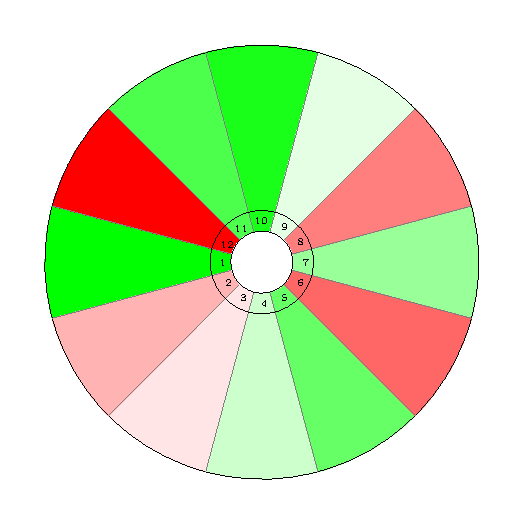
\includegraphics[width=0.7\textwidth]{diagrams/superior-places}
\vspace{-1em}
\caption{The Superior Places}
\end{figure}
\begin{mdframed}[backgroundcolor=cyan!5, rightmargin=1em, leftmargin=1em]
\small
In the figure the seven \textsl{good} places are in shades of green; the bad in shades of red.
\end{mdframed}
\section{Power of the Seven Planets}

Every planet in its own sign, exaltation, or triplicity is benefic as ``what it indicates of good is strong, increasing.'' This is true even of malefics as their ``evil becomes lighter and decreases'' when they are in their own places.

\Saturn\, in a masculine sign\footnote{In \S1.4 we are told \Saturn\,(a diurnal planet) is at his worst when in a feminine sign. Here we are told he can still do harm when in a masculine sign but not as much and even less if he is in one of his own dignities. In the same section, \Mars\, (a nocturnal planet) in a feminine sign is described as less harmful than a feminized \Saturn.} in a day chart (even though he is a diurnal planet) can cause harm but it will be less harmful if he is also in one of his own dignities. The same is true for \Mars, a nocturnal planet, in a feminine sign in a nocturnal chart. 

A planet's power \textsl{disappears} if it is within 15° of the \Sun\, while the \Sun\, is moving towards a conjunction with the planet.

A retrograde planet indicates ``there is difficulty [and] misfortune'' for the person and others.


\section{More on Upbringing}

\subsection{Good Upbringing}
\label{sec:upbringing2}
The person will be brought up if diurnal planets in a diurnal chart or nocturnal planets in a nocturnal chart are found in:
\begin{itemize}[topsep=0pt,itemsep=0pt]
\item one or more of the seven strong places; it is beneficial if one of them is a benefic

\item the 2nd place from the ascending sign if the planet is within 15° of the Ascendant as then ``reckon its power as if it were in the ascendent''
\end{itemize}

\subsection{No Upbringing}
The person may not be brought up or have a harsh upbringing if:
\begin{itemize}[topsep=0pt,itemsep=0pt]
\item the first triplicity ruler is within 15° of the \Sun\, or in a bad place; especially if the second triplicity ruler is with him

\item both malefics aspect the \Moon, especially if she is in an angle and one of the malefics is in opposition while also making an exact aspect to the Ascendant\footnote{Dykes indicates it could be an aspect to the Ascendant's terms rather an exact aspect to the Ascendant's degree (CAD p.69).} as ``this is an indications of ruin''

\item the \Moon\, in the 7th place with no connection to a benefic and while a malefic is in an angle for ``then the women give birth to what has no escape from ruin''

\item the \Moon, not in her own places, in the 4th with \Saturn\, and \Mars\, or in their opposition

\item one of the malefics in the Ascendant opposite the other malefic and the \Moon\, in the 10th or 7th

\end{itemize}

\subsection{Rejection or Exposure}
The person may be cast out by his parents if:
\begin{itemize}
\item the \Moon\, in the 4th place with \Saturn\, and \Mars\, or in their opposition unless the \Moon\, is in her own triplicity and the benefics are trine the malefics in which case, rather than ruin, the person is brought up by strangers and sometimes they ``will be a slav and will be employed and then will be miserable''

\item the \Moon\, ``between the two malefics and one them casts its rays upon it'' then the person's livelihood will be little and if the \Moon\, is also waning ``it indicates fate and shortness of life'' which he may escape if a benefic is also part of the configuration

\item the \Moon\, is with a malefic in an angular or succedent place and is configured with a benefic and if the \Sun\, aspects the malefics, the father favours casting him out and thinks badly of him; if the \Moon\, is injured\footnote{This is odd as we've already been told the \Moon\, must be with a malefic, which would be an injury; possibly it must also be harmed by the other malefic?}, the mother wants to cast the person out; if both lights are injured, both parents want rid of the person

\item in a diurnal chart, \Mars\, angular and opposing the \Moon\, or the \Sun\, while they are not in their own places; in a nocturnal chart, \Saturn\, under the same conditions
\end{itemize}

\subsection{Calamity}

If the \Moon\, is in the term of a malefic without the aspect of a benefic while a malefic is in an angle there is ``calamity'' for the person unless first ruler of the sect light's triplcity aspects the \Moon.

\subsection{Injury to the person and his mother}

If there is no benefic in (a) an angle, (b) in the same sign as the Lot of Fortune, or (c) in a sign of the same triplicity as the Ascendant while malefics aspect the \Sun, \Moon, and SAN\footnote{The most recent new or full moon that occurred prior to the birth.} the indications are evil.

If a benefic does not aspect the Ascendant (representing the person) or the \Moon, an unfortunate condition is indicated for the person and their mother if the \Moon, or worse yet, the \Moon\, and \Venus\, (as both indicate the mother) are injured.

\textsl{\small(also see \S\ref{sec:upbringing} Upbringing and \S\ref{sec:upbringing3} Upbringing Again, \S\ref{sec:upbringing4} Upbringing and Livelihood)}
\section{Masculine and Feminine Hours}

The person represented by the chart will be a male if:
\begin{itemize}[topsep=0em, itemsep=0em]
\item the  \Moon\, is in a masculine dodecatemorion
 \newline\newline
To determine the dodecatemoria divide the sign into 2.5° sections\footnote{Dorotheus says ``two and a half days'', we are basically dividing the 30° of each sign by 12 so it has an analogy with each month of 30 days being equivalent to a sign and the 12 signs being equivalent to a year.} with, in a masculine sign, the sections running male, female, male, female, etc. In a feminine sign, the sections running female, male, female, etc\footnote{For more information on the  \textsl{dodecatemoria}  and their calculation see the Appendix  \textsl{\S\ref{appendix:dodecatemoria} Dodecatemoria}.}

\item the \Sun, \Moon, and Ascendant are all in masculine signs

\item the \Sun\, in the ascendant in a masculine sign, even if the hour of the birth is ``double'' (even)

\item a masculine planet in the ascendant in a ``two-bodied'' masculine sign (\Gemini, \Sagittarius), even if the hour of the birth is ``double'' (even)

\item a masculine planet in the 1st and in the 7th,  even if the hour of the birth is ``double'' (even) 

\item the \Sun\, and \Moon, both in masculine signs, and \Jupiter\, ruling the Ascendant regardless of gender of the sign on the Ascendant

\end{itemize}	
\section{Upbringing Again}
\label{sec:upbringing3}

Also look to see if the \Moon\, is with or aspecting either the Lot of Fortune or the Lot of the Demon as this is an indication the person is well brought up and has a beautiful face, fine limbs, and any easy time teething. If the \Moon\, has no connection with either lot then say the reverse.

\textsl{(also see \S\ref{sec:upbringing} Upbringing and \S\ref{sec:upbringing2} More on Upbringing)}				% masc/fem hours
\section{Is the Person and their Mother Free or a Slave}

First, examine the \Moon's condition. 

If the \Moon\, is in the 12th or 6th place and:
\begin{itemize}[topsep=0em, itemsep=0em]
\item the first triplicity lord of the place is in a bad place, the native is a slave, unless
\begin{itemize}[topsep=0em, itemsep=0em]
\item it is a night chart and the \Moon's second and participating triplicity lords are in good places, or
\item it is a day chart and the first and second lords of the \Sun's tripicity are in good places
\end{itemize}
In which case the person is born free but his parents are poor.
\end{itemize}

If the \Moon\, is in the last degrees of a sign, the mother is of bad descent unless:
\begin{itemize}[topsep=0em, itemsep=0em]
\item  \Jupiter's aspect removes the misery, which happens even if \Jupiter\, is badly placed\footnote{The wording in the original is confusing; this appears to be the author's intent.}, or

\item the \Moon\, is with \Venus\, in one of \Venus's domiciles in which case ``the evil'' disappears.
\end{itemize}

If a malefic is in one of the \Moon's angles\footnote{If either malefic found in the 4th, 7th, or 10th place from the \Moon.} and \Mars\, (in a day chart) or \Saturn\, (in a night chart) aspect the \Sun\, or \Moon\, without \Jupiter\, also being in aspect, the person will be a servant. And his condition may be worse if the \Moon\, is in a feminine sign and worse yet if \Venus\, is also injured.

If the \Sun\, and \Saturn\, are in the 6th, 12th, 8th, or 4th then the father's condition is unfortunate.

If the \Sun\, and \Moon\, are in the terms of benefics and aspect the ruler of the place they occupy then the parents condition is good as will be the person's survival and upbringing. The conditions will be even better if  the \Sun\, or \Moon\, is angular or it one rules the Lot of Fortune.

If the \Moon\, is angular or succedent and being overcome\footnote{The text has ``supervised'', Dykes translation has ``looked down on'' which he equates with \textsl{overcoming}.} by a malefic, the person will be struck down even if he is free. There is destruction if the \Moon\, is with one malefic while ther other overcomes them.

In a nocturnal chart, if the \Moon\, is in the 7th or 4th and in the aspect of a malefic, destitution, slavery and difficulty is indicated for the persons livelihood.

The Lot of Fortune or its ruler in another's terms is in the 6th or 12th  indicates service.

If the \Moon\, in a nocturnal chart is in a masculine sign while the Ascendant is in a feminine sign or, if in a diurnal chart, the \Sun\, is in a feminine sign while the Ascendant is in a masculine sign, the person will be like a slave.

Check the \Moon's, \Sun's and Ascendant's term rulers to see if they are feminine (\Saturn, \Venus\, \Moon) or masculine (\Sun\, \Jupiter, \Mars)\footnote{This is strange for a number of reasons (1) Dorotheus does not connect the state to the condition of being free or a slave, (2) the \Moon\, and the \Sun\, do not rule any of the the most commonly used Egyptian terms, (3) \Saturn\, is usually considered a diurnal and therefore masculine planet although Dykes says there are other instances of \Saturn\, being deemed feminine found in Sahl and Theophilus.}.

The \Moon\, with the malefics without the aspect of a benefic indicates slavery.

A malefic in an angle or \Mars\, aspecting the \Moon\,  while the \Moon\, is moving to conjunct \Saturn\, indicates slavery. The same if \Saturn\, is aspecting the \Moon\, while is moving to conjunct \Mars.

If the \Moon\, is in the end of a sign and aspected by \Saturn\, or \Mars\, the person may be aborted or his birth made hard; unless \Jupiter\, or \Venus\, also aspect the \Moon, in which case the person is born but raised by strangers.

If the first lord of the Ascendant's triplicity is cadent and opposed by the \Moon\, while the \Sun\, is in a bad place, the person's parents are slaves.

\subsection{Indications from the SAN}

Note the degree of the SAN\footnote{SAN is an acronym for \textsl{Syzygyium Ante Nativatem} which refers to the \textsl{syzygy}, the whole-moon (conjunctional) or full-moon (prevtional) immediately before birth which may also be called the \textsl{lunation} before birth.} and the 1st and 2nd triplicity lords of its sign. 

If the 1st lord is in a bad place and the 2nd in a good place, the person will be born into slavery but freed in later life.

If the 1st lord is in a good place and the 2nd in a bad place, the person is born free but will be reduced to poverty, contempt and service in his later years.

If both triplicity lords are bad places, the person will being and end life as a slave or servant.

If both triplicity lords are in good places, the person will begin life free and end it free.

If a malefic is with the SAN and the other malefic is in aspect, the person ``will experience his fate and evil will overcome him.''

If the SAN's term lord is in a bad place or the 7th or the 4th the life will be lived in slavery and poverty.

If the SAN is in a bad place and aspected by malefics but it is also aspected by a benefic and its term lord is in a good place then the person's father if os noble birth and his mother is of poor lineage.

\subsection{Escape from Slavery, Service, or Poverty}
Indications that a person will be freed from any indicated slavery, service, or poverty are:
\begin{itemize}[topsep=0em, itemsep=0em]
\item \Jupiter\,  in any angle, in any sign except \Capricorn, regardless of being with malefics or benefics. And if \Jupiter\, aspects the \Moon, ``the pains of slavery are completely loosened for him.''

\item \Venus\, in an angle, free of the malefics

\item \Venus\,  in the 7th with the \Moon

\item the \Sun, \Moon, and \Mercury\, in angles
\item the \Sun\, and \Moon\, in the same triplicity
\item the \Moon\, angular in \Taurus\, or \Cancer\, free of the malefics or aspected by both malefics and benefics
\end{itemize}

\subsection{Effect of Jupiter}
If \Jupiter\, is with or square the Lot of Fortune the person escapes slavery but if \Jupiter\, aspects the Lot of Fortune while both are  in bad places the person will be freed from slavery but will not escape servitude.

If \Jupiter\, is in the 2nd or 8th the person will experience what is like slavery and worse if \Jupiter\, is in the 6th or 12th.























\section{How many will own the person}

In a day chart, if slavery is indicated, to know how many will own the person count the planets between the \Sun\, and the lord of the triplicity of the Lot of Fortune. In a nocturnal chart count from the \Moon\, instead of the \Sun.

If the \Moon\, is above the earth count the planets between the 6th place (the sign of slaves) to the 12th place and if the \Moon\, is under the earth, count the planets between the 12th and the 6th.

And if any planet is in a double-bodied sign (\Gemini,\Virgo, \Sagittarius, \Pisces) count it as two planets instead of one.

To know how many would own the father, count from the \Sun\, to the lord of the \Sun's triplicity, and for the mother, count from the \Moon\, to the lord of the \Moon's triplicity.


\section{Upbringing and Livelihood}
\label{sec:upbringing4}
\subsection{Moon on the 3rd Day after Birth}
Check the sign the \Moon\, is in on the third day after birth and consider:
\begin{itemize}[topsep=0em,itemsep=0em]
\item the place the sign occupies
\item the planets aspecting the sign
\item the place and condition of the sign's domicile  and exaltation rulers
\end{itemize}

\noindent The person's condition is good and fortunate if:
\begin{itemize}[topsep=0em,itemsep=0em]
\item the places occupied are good and in the aspect of benefics
\end{itemize}

\noindent The person's condition is middling, he is ``neither happy nor destitute'' if:
\begin{itemize}[topsep=0em,itemsep=0em]
\item the domicile ruler is in a good place, not USB, or in the aspect of benefics
\end{itemize}

\noindent The person's condition is miserable if:
\begin{itemize}[topsep=0em,itemsep=0em]
\item the places occupied are bad and aspected by malefics
\item malefics aspect the domicile ruler
\end{itemize}

\subsection{Indications from the radix Moon}
The person's condition is good if:
\begin{itemize}[topsep=0em,itemsep=0em]
\item the dodecatemoria of the \Moon\, with benefics or in their aspect\footnote{This is implied from his comments on the dodecatemoria causing misery.}

\item the \Moon\, is waxing and moving North\footnote{It is not clear if this is North in latitude or North in the sense that Valens describes it under winds in Book 3.4.} the person ``attains good at the end of his life''

\item the \Moon\, ascending, moving from South to North, then ``he attains good at the beginning of his life and at the end''; it is best if 

\item it is best if the \Moon\, waxing and ascending North as it is an indication of prosperity and virtue
\end{itemize}

\noindent The person's condition is unfortunate if:
\begin{itemize}[topsep=0em,itemsep=0em]
\item the dodecatemoria of the \Moon\, with malefics or in their aspect
\item the \Moon\, is void\footnote{There are two current ideas of what what determines if the \Moon\, is \textsl{Void of Course}. The most widely used interpretation is the \Moon\, not applying to aspect any planet within the next 30° of her travel. Others limit it to her not applying to the aspect of another planet while she moves through the sign she occupies at birth.}, no planets in or aspecting the Ascendant\footnote{Dykes has the \Moon\, not in or aspecting the Ascendant.}; the  person will possess ``pain and hardship in the pursuit of what he needs''
\item the \Moon\, is waxing and is \Conjunction, \Opposition, or \Square\, to \Mars
\item the \Moon\, is waning and is \Conjunction, \Opposition, or \Square\, to \Saturn
\end{itemize}

\subsection{Indications from the 10th Place from the Moon}

If there is a benefic in the 10th place from the \Moon, there is good for the person. If the benefic is in their own places then the person ``attains wealth and gains in right and honesty.''

If there is a malefic in the 10th place from the \Moon, the good is less and if the malefic is not in his own places then the indication is for ``great harm.''

\subsection{Indications for the Parents}
The \Sun\, and his triplicity rulers indicate the father and his end and the \Moon\, and her triplicity rulers indicate the mother, her end, and the native. The lord of the 4th is also an indicator for the parents.

If the \Sun\, and his triplicity lords and the \Moon\, are in bad places then both the mother and father will have ``misery and little livelihood'' and that the person ``will not be brought up'' but harmed by his parents. If, at the same time, there is a benefic in an angle, the misery will be held off for a period equal to the benefic's minor years.

If the \Sun\, is in a good place with the aspects of both malefics and benefics, it indicates a doubling of the father's property ``but also the diminuation of the property'' of the person. The same happens re: the mother if the \Moon\, is in a similar condition. And the loss will be worse if the ruler of the 4th is also harmed.

If the \Sun\, and/or \Moon\, is cadent and aspected by malefics then the father, or mother, or both are slaves, living in poverty and in need of ``nourishment day by day'' and if, along with this, the Ascendant ruler is also cadent ``then the native is not brough up out of misery and expulsion because he is a slave or a pauper or one in need of nourishment.''

\subsection{Indications for the Father from the Sun}

If the \Sun\, and the \Sun's first triplicity ruler are in good places then:
\begin{itemize}[topsep=0em, itemsep=0em]
\item wealth, praise, and fame is indicated for the father
\item it is better if the \Sun\, is also in the terms of a benefic as it means the person will inherit from their father
\item if the triplicity ruler is with a malefic there is an decrease in the father's property and ``injuries and calamities''
\end{itemize}

\noindent If the \Sun\, and the \Sun's first triplicity ruler are in bad places then:
\begin{itemize}[topsep=0em, itemsep=0em]
\item the father ``is not noble and poverty and necessity have overtaken him''
\end{itemize}

\noindent If the \Sun\, is in a good place but the first triplicity ruler is cadent, then:
\begin{itemize}[topsep=0em, itemsep=0em]
\item the father ``is noble, but he will not keep his property and honor''

\item if the \Sun\, is also in the term so malefic, his father ``has no splendor because [this is] an indication of service for him'' and if a malefic  also aspects the \Sun,  there will also be illness for his father
\end{itemize}

\noindent If the \Sun\, is iin a bad place but the first triplicity ruler is in a good place, the father increases and both the person and his father are elevated over their peers.

If the first triplicity ruler of the \Sun\, is in a strong place and the second triplicity ruler is in a bad place, his father is in good condition when the person is born but they do not persist; and the reverse is  true if the first triplicity ruler is in a bad place and the second in a good place.

The \Sun\, and its first triplicity ruler in a bad place, in its ``dejection'' or other signs not its own, ``then it indicates death in a terrible place for his father'' and if, at the same time, a malefic is \Square\, or in \Opposition, ``all the property of his mother and father will be squandered.''

\subsection{Indications for the Mother from the Moon}
Things are bad for the mother if:
\begin{itemize}[topsep=0em, itemsep=0em]
\item the \Moon\, is descending South, or
\item in an eclipse, or
\item in the terms of a malefic, or
\item in its \textsl{dejection} (Fall?)
\end{itemize}
and if a malefic also aspects the \Moon, it is worse.

If the \Moon\, is in the terms of a benefic and any of the above conditions apply, then ``the mother is noble, but ignominy and disdain and humiliation have struck her.''

If the \Moon\, is in the 4th ``a chronic illness will strike [the] mother or she will be harmed in her reputation.''

If the \Moon\, is in the 4th or 7th, in the terms of a malefic, and her dispositor is cadent, she ``is in slavery.''

If the \Moon\, is angular and is in \Conjunction, \Square, or in \Opposition\, to \Saturn\, or \Mars, then the person's mother ``will die a terrible death.''

If the \Moon\, and her triplicity rulers are in bad places, and the \Sun\, and its triplicity rulers are in good places then the mother has a bad end but not the father.

\textsl{\small(also see \S\ref{sec:upbringing} Upbringing, \S\ref{sec:upbringing2} More on Upbringing, \S\ref{sec:upbringing3} Upbringing Again)}
\section{Lot of the Father}

Calculate the Lot of the Father, by degrees, in a day chart from the the \Sun\, to \Saturn; for a night chart, count from \Saturn\, to the \Sun\,. Add the degrees found to the Ascendant, the result is the place of the lot.

If \Saturn\, is USB, use from \Mars\, to \Jupiter in place of \Saturn\, and the \Sun.

If the lot ruler is in any of the good places, then the father's condition is good; if it is in the 6th, 8th, 3rd, or 12th\footnote{Probably should include the 2nd place as well.} his father's condition is bad.

If the lot's ruler is in the sign following the lot\footnote{In the 12th sign from the lot.}, not aspecting\footnote{Pingree's text omits the ``not'' but that would contradict what Dorotheus said about the condition of the father being good if the lot ruler is in a good place, all of which would aspect the lot.} the lot, or if the ruler of the sign opposite the lot is in the lot, then the person's father is not his real father.

							% Lot of the Father
\section{Lot of the Mother}

Calculate the Lot of the Mother, by degrees, in a daytime birth, from \Venus\, to the \Moon; for a night chart, from the \Moon\, to \Venus, and add the difference found to the Ascendant.

The parents are of different nationalities if:
\begin{itemize}[topsep=0em, itemsep=0em]
\item the \Sun\, and \Moon\, are both in tropical signs (\Aries, \Cancer, \Libra, \Capricorn), especially if the malefics are conjunct, square, or in opposition to them

\item the lights don't aspect each other or the Ascendant

\item one of the lights is below the earth, the other above with malefics

\item the Ascendant is in a tropical sign with one of the lights and there are other planets with them, especially a malefic
\end{itemize}

\subsection{Separation of Parents}
The \Sun\, or \Moon\, in the 7th place indicates the parents are separated and, if the light is in the terms of a malefic, the indicated parents property is squandered.

\Mars\, or \Saturn\, conjunct, square, or opposed to the \Sun\, without any aspect from the benefics indicates the father's property is squandered. If the \Moon\, is in the same position, the mother's property is squandered. And if the parents are separated when the person is young he may be a needy orphan.

\Saturn\, angular, especially in the 7th,  with \Jupiter\, cadent and not aspecting \Saturn\, indicates separation of the parents. The same if \Mars\, is in the same condition and \Saturn\, and \Venus\, in the same condition as \Jupiter.

The two lights opposed to each other across the 6th-12th axis, or both together in the 6th or 12th, indicates the parents separation.

The lot of the father and mother together in the same place indicates separation of the parents as do malefics aspecting the lots.

Separation is also indicated if the two lights do not aspect each other or the Ascendant.

``If you find the two lots, each one of them, in a sign at its term[s], and the malefics are also injuring them from the sign, then this is an indicator of the destruction of what is between the parents.\footnote{Can't make head or tails of this. Dykes has ``And if you found the two Lots, each of them in a sign separated [from the other]\textsl{[in aversion]}, and the infortunes also harming them both from the sign\textsl{[possibly the 4th or 7th is meant]}, then that is an indicator of the corruption of what is between the parents.'' I am wondering if it might mean if you find the lots in the terms of a malefic and also harmed by the same malefic.}.''

\subsection{The 4th Place}
The \Moon\, and \Venus\, both aspecting the 4th indicates ``an increase of good and a goodness of condition'' for the mother.

If the \Sun, \Jupiter, and \Saturn\, are in the 10th in opposition to the 4th ``it indicates praise of the father and the goodness of his condition.'' 

If both the above situations occur at the same time ``then judge for his two parents together good fortune and wealth and fame.''

Misfortune, misery, and slavery for the parents is indicated if \Mars\, and \Saturn\, are in the 4th without a benefic or if the malefics square or oppose the 4th.

The \Moon\, in the 4th indicates evil for the mother; the \Sun\, in the 4th, evil for the father.



						% Lof of the Mother
\section{Parent Deaths}

Indications of which parent will probably die first:
\begin{itemize}[topsep=0em,itemsep=0em]
\item the parental lot that contains a malefic or is in its square or opposition

\item \Mars\Square\Sun\, from the left\footnote{Dykes says ``That is, overcoming the \Sun'' althoug usually ``overcoming'' is described as on the ``right''; essentially, the \Mars\, must be in square from the 10th from the \Sun, not square in the the fourth sign from the \Sun.}, the father is indicated; if the \Moon\, is in a similar situation, then the mother is indicated

\item \Mars\, in the 2nd place from the \Sun\, (indicates the father) of the \Moon\, (indicates the mother)

\item the \Sun\, (father) or \Moon\, (mother) square or opposed to a strong malefic

\item if both the Lot of the Mother and the Lot of the Father are in the square or opposition of malefics without the aspect of the benefics\footnote{The text has ``but [the two lots] not aspecting any of them [the malefics]'' but that makes little sens; Dykes has ``and $<$the fortunes$>$ not looking at them'' (the lots).} see which of the \Sun\, or \Moon\, will first enter the 4th place by diurnal motion

\item if both the lights are injured by malefics look to the SAN ``as this will indicate to you whatever of that you wish''\footnote{He doesn't say which parent is indicated by the new or full \Moon.  New \Moon, mother?}

\item if a light is below the horizon and malefics aspect the Ascendant then the parent indicated by the light will die first
\end{itemize}

\Saturn\Opposition\Mars\, or \Mars\, overcoming \Saturn\,  is an indication the father's property will be destroyed.

The time of death is shown by the lots. If \Saturn\, transits the lot and \Jupiter\, is in an angle, the person will inherit their father's property at his death.

If \Saturn\, and \Mars\, transit the sign where both lights are then both parents will die.
\section{Person's Inheritance}

\subsection{The Father's Property}
The father's property is indicated by the \Sun\, and \Saturn.

In a day chart, if they are both in good places, the person will inherit his father's property. He will also hold on to it if  the benefics aspect the \Sun\, alone or both the \Sun\, and \Saturn.

If  \Mars\ is \Square\, the \Sun\, the person will squander his inheritance. 

The person will waste his father's property both before and after his father's death if the \Sun\, is in the 6th or 12th, or, \Mars\, is in an angle and especially if, in a day chart, \Saturn\, is in his dejection\footnote{Probably means \Saturn\, is in his Fall (\Aries).}. The grief from the loss will be mitigated if \Jupiter\, aspects.

The father will die a terrible death if:
\begin{itemize}[topsep=0em,itemsep=0em]
\item the lord of the Lot of the Father is in a bad place and in the aspect of a malefic posited in the 4th or 7th.

\item the lord of the Lot of the Father in a bad place and neither the \Sun\, nor the lord of the \Sun\, aspecting the Ascendant
\end{itemize}

Indications for the relationship between a father and son:
\begin{itemize}[topsep=0em,itemsep=0em]

\item  \Jupiter\, overcoming \Saturn; the father will be miserable because of his son.

\item \Jupiter\Opposition\Sun; ``misery and misfortune'' between the father and son

\item \Saturn\, in the triplicity of \Jupiter; they love each other and the son will inherit his father's property
\end{itemize}

\subsection{The Mother's Property}
The mother's property is shown by the \Moon\, and \Venus\, and their lords.

The the \Moon\, and \Venus\, are in the west, in a bad place, and the \Sun\, is cadent without a good aspect to relieve the \Moon, \Venus, or the bad place then the person is born to parents who are poor and needy, and so is the person.




\section{Number of Siblings}

To know how many siblings were born before the person examine the Ascendant's triplicity rulers and see where the stronger one falls in the chart:
\begin{itemize}[topsep=0em, itemsep=0em]
\item in the 1st, the person is the first\footnote{Dorotheus says ``the cardines indicate the beginning.''} born
\item in the 10th, the person is the fourth born or the first born
\item in the 7th, he is the seventh child or the first
\item both triplicity rulers cadent, ``sometimes nothing is allotted''
\end{itemize}

If both the triplicity rulers are on the left side of the Ascendant, look at what is between the triplicity rulers and the Ascendant:
\begin{itemize}
\item a malefic indicates the mother had a miscarriage or that a sibling born before the person has a birthmark or defect
\item a benefic, direct, rising from the \Sun, indicates there will be more siblings than predicted
\item if no planets are found in-between, the person is the first born and if they are not, it indicates the sibling born before them was a miscarriage or will die before them
\end{itemize}

If there is a planet between the Ascendant and the IC there will be a sibling born after the person and if that planet is a malefic, they will die. If there are no planets found, there are no siblings born after the person.						% how many siblings
\section{On Brothers}
A person with the Ascendant or \Moon\, in \Leo\, or \Sagittarius\, will have few brothers.

\Mercury\, in a term of \Mars\, aspecting the \Moon\, or the Ascendant is harmful to brothers.

If the Ascendant is in \Scorpio, \Cancer, or \Pisces, the mother will have numerous children.
\section{Lot of Brothers}

To find the Lot of Brothers count (in the order of the signs) from \Saturn\, to \Jupiter\, by day or \Jupiter\, to \Saturn\, by night and add the difference to the Ascendant. A planet in or aspecting the lot will make clear matters concerning the brothers.

If the lot is in sterile signs (\Leo, \Virgo, \Capricorn) ``there is not good in his brothers'' while if it is in \Cancer, \Scorpio, or \Pisces, he will have numerous brothers.

\Jupiter\, and \Venus\, aspecting the lot, even by square, indicates good things in the matter of brothers.

\Mars\, or \Saturn\, aspecting the lot by square or opposition injures and diminishes the brothers and sometimes indicates they will die before the person. But if the malefics aspect by trine or sextile ``there is no great calamity'' for the brothers.






\section{Brother's Love}

To know if the brothers love each other or otherwise, look at the lord of the Lot of Brothers, if it aspects the lot by:
\begin{itemize}[topsep=0em,itemsep=0em]
	\item[\Trine] there is love between brothers
	\item[\Square] there is  ``a medium amount of love.''
	\item[\Opposition] there is ``enmity and separation''
	\item[\Semisextile] there is estrangement between them
	\item[\Quincunx] there is estrangement between them
 \end{itemize}


\section{How many siblings?}
To find the Lot of the Number of Siblings\footnote{Note that \textsl{siblings} is being used here and elsewhere in place of \textsl{brothers}.}, count (in the order of the signs) from \Mercury\, to \Jupiter\, (by night, from \Jupiter\, to \Mercury) and add the difference to the Ascendant. The number of planets aspecting the place of the lot gives you the number of siblings.

Indications from the planets aspecting the place are:
\begin{description}[labelindent=0em , labelwidth=6em, labelsep=0.5em, leftmargin =!]
\item [\Venus,\Mercury] in aspect from a good place, from feminine signs indicates sisters; in masculine signs, brothers

\item[\Saturn,\Mars,\Sun\,\Moon] peregrine, indicate the loss of siblings but if in their own places his siblings ``will not love him and are not his friends or who have no use for him because what the malefics indicate is not complete''

\item[any planet] in aspect from a bad place indicates the siblings ``have no good in them or have sicknesses, or that there is enmity between them, and bad and evil [are their] opinion and thought [of each other]
\end{description}

\subsection{Indications from the 3rd Place}
If the sign on the 3rd place is double-bodied (\Gemini, \Virgo, \Sagittarius, \Pisces) or its lord is in a double-bodied sign then the siblings are not the children of both parents.

Indications from the planets as to birth-order:
\begin{itemize}
\item[\Saturn,\Mars] older brothers
\item[\Jupiter,\Mars] middling brothers
\item[\Mercury] younger brothers
\item[\Moon] older sisters
\item[\Venus] younger sisters
\end{itemize}

\subsection{General Indications from Mars}
If the 1st and 2nd triplicity rulers of \Mars\, are in bad places, it indicates a small number of siblings.

If one triplicity ruler is in  a good place and the other in a bad place then the person has siblings ``but it is inevitable that he will see their death.''

\vspace{-1em}
\begin{figure}[H]
\centering
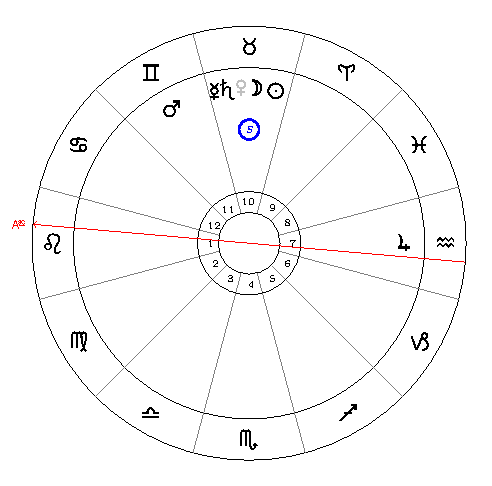
\includegraphics[width=0.7\textwidth]{charts/1_01}
\vspace{-1em}
\caption{Chart 01: Man with 5 Siblings}
\end{figure}

The chart of a man with the \Sun, \Moon, \Saturn, \Mercury\footnote{\Venus\, is missing from the original chart, Dykes places it in the 10th, dating the chart to May 2 or 3, 29 AD JC, $\approx$ 11:30AM Sidon, Lebanon.}, and the Lot of Siblings in the Midheaven in Taurus with \Mars\, in \Gemini, \Jupiter\, in \Aquarius, and the Ascendant in \Leo.

\Saturn\, and \Mercury\, are the indicators of siblings as they are the triplicity rulers of \Mars\, (the general indicator of siblings). ``Because they both happen to be above the earth you count from them to the ascendent, but if they were below the earth you would count from the ascendent to them.''

Predict the person will have five siblings as the two triplicity rulers are in \Taurus\, and counting from there to the ascendent sign of \Leo\, gives: \Taurus\, (1) + \Gemini\, (double-bodied gives 2) + \Cancer\, (1) + \Leo\, (1) = 5.

If both the triplicity rulers had not been in one sign it would be necessary to take the count from whichever was eastern and in a strong place, or, if both were of equal strength, to start the count from the day or night triplicity ruler (depending on the chart sect). 

The Lot of Siblings is in a feminine sign (\Taurus) with \Saturn\, indicating his sister will die, as will both an older and his youngest brothers because the \Sun\, and \Mercury\, are also with the lot and \Saturn\, in \Taurus\, but the fullest effect of these will not be felt because \Jupiter\, aspects the place\footnote{An example of the \Square\, of \Jupiter\, being beneficial rather than harmful when he is angular and in one of his own places (he's the participting triplicity ruler of \Aquarius).}
\section{The Native's Fortune, Property and Illness}
To discover the utmost limit of the native's fortune and status, look at the sect light and its triplicity lords.

If the 1st and 2nd lords are in good places ``then his condition will not cease from the beginning of his age to the end of his life to be in excellence and elevation and wealth.''

If the 1st is in a good place and the 2nd in a bad place ``then his condition will be better in the beginning of his age, but will degenerate at the end of his life.''

If the 1st is in a bad place and the 2nd in a good place ``then it indicates middling good in his life, but this will not last in him.''

If the 1st is in a bad place and the 2nd is under the earth or in a bad place, ``then some misfortunes reach him and he does not have every desire, but some forbearance against calamity and grief and loss in livelihood is inevitably his.''

If you find both cadent, ``then this will not cease being in mesery and poverty, especially if the malefics aspect thse two from quarile or opposition and the malefics are in cardines; whoever is thus will not find bread to fill his belly or clothes in which to clothe himself.''

If the triplicity lord is USB or in the place of \Saturn, ``then whatever of good it indicates is not stable,a nd his property will not increase, and he will be more learned in meditation than he is in work.''
\section{Good and Evil Planets}
In a bad nativity, if \Jupiter\, is in an angle, ``then it will drive off the evil for twelve years'' but if it is in a succedent place, ``it will obstruct  the calamity until it reaches a sign in which \Jupiter\, indicates calamity.''

\Venus\, angular, ``will obstruct [evil] for eight years.''

\Saturn\, angular and dominant (being a triplicity ruler of the sect light), ``will obstruct [evil] for thirty years.''

\Mercury\, angular and dominant, ``will obstruct [the evil] in a nativity like this for twenty years.''

\Mars\, angular and dominant, ``will obstruct [the evil] for fifteen years.''

The \Sun\, angular or in its own triplicity in a day chart, ``will drive off the evil for nineteen years.''

The \Moon\, angular in a feminine sign, ``will drive off the evil for twenty-five years, but in a masculine sign, for twenty-five months.''

\section{Judgments (Example Charts)}
Examples of judging a person's fortune and property primarily from the placement of the sect light's triplicity rulers.

\begin{figure}[H]
\centering
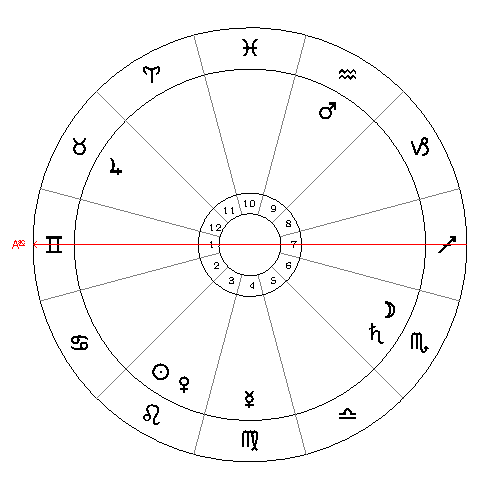
\includegraphics[width=0.7\textwidth]{charts/1_24_01}
\vspace{-1em}
\caption{Chart 02: Needy, Poor, Miserable}
\end{figure}

The nativity is nocturnal and the triplicity rulers of the \Moon\, in \Scorpio\, are first \Mars, second, \Venus. As both are cadent, ``this man should be needy, poor, not finding his daily bread, miserable. And this was in him more evident than what I told you.''

\begin{figure}[H]
\centering
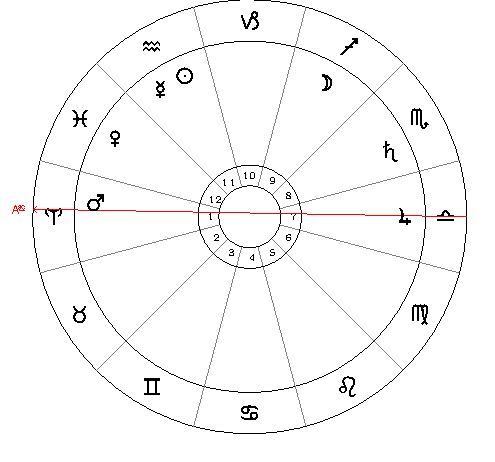
\includegraphics[width=0.7\textwidth]{charts/1_24_02}
\vspace{-1em}
\caption{Chart 03: Wealthy, Rich, Powerful}
\end{figure}

The nativity is diurnal and the triplicity rulers of the \Sun\, in \Aquarius\, are first, \Saturn, second, \Mercury; both in succedent places. \Mercury\, is in ``the place of fortune, so that the native should be wealthy, rich, powerful in business affairs, great in property, seizing eminence and fortune and increasing in them.''

\newpage
\begin{figure}[H]
\centering
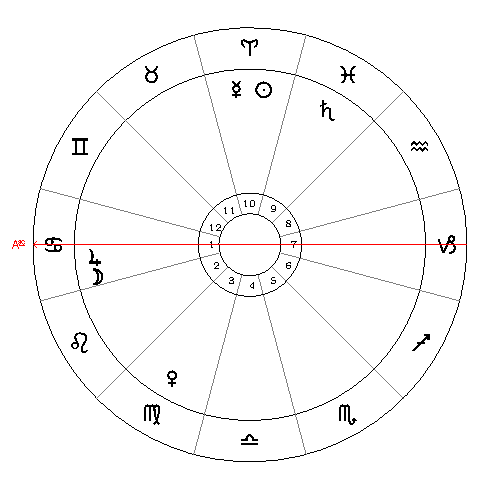
\includegraphics[width=0.7\textwidth]{charts/1_24_03}
\vspace{-1em}
\caption{Chart 04: Praised by kings, nobles, wealthy men}
\end{figure}

The nativity is diurnal\footnote{The position of \Mars\, was not given.} and the triplicity rulers of the \Sun\, in \Aries\, are, first, the \Sun, second, \Jupiter, both of which are in angles and in their own exaltations ``so that the native should be praised with the praise of kings and nobles and wealthy men.''

He will be ``praised with the praise of kings'' because \Saturn, the third triplicity ruler, is cadent in \Jupiter's sign (\Pisces) in trine to \Jupiter\footnote{\Saturn\, is in the 9th place which the Greeks associated with royalty.}.

\begin{figure}[H]
\centering
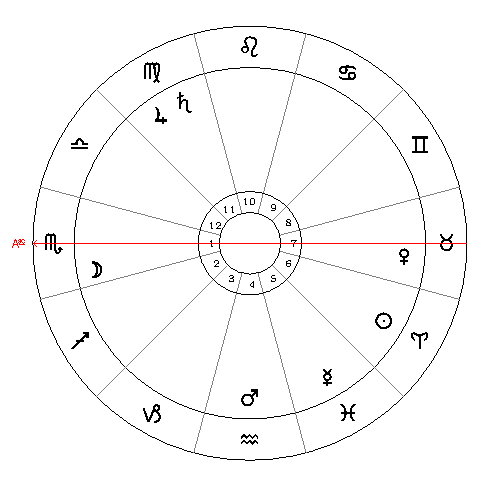
\includegraphics[width=0.7\textwidth]{charts/1_24_04}
\vspace{-1em}
\caption{Chart 04: Eminent, powerful, praised}
\end{figure}

The nativity is nocturnal and the triplicity rulers of the \Moon\, in \Scorpio\, are, first, \Mars, second, \Venus, third, the \Moon. As all three are angular ``this man is mighty in eminence, powerful in leadership so that crowns of gold and silver are placed on him and he is praised.''

\newpage
\begin{figure}[H]
\centering
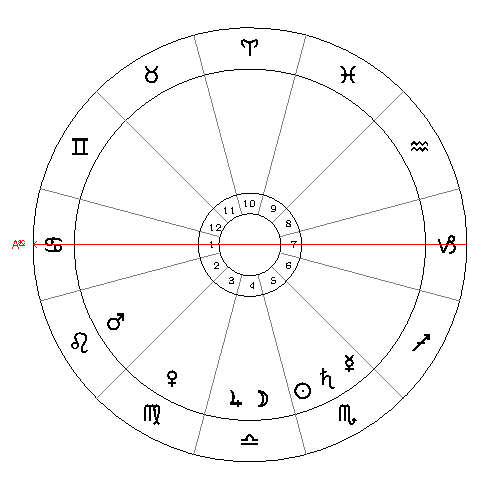
\includegraphics[width=0.7\textwidth]{charts/1_24_05}
\vspace{-1em}
\caption{Chart 05: Poor, unfortunate}
\end{figure}

The nativity is nocturnal and the triplicity rulers of the \Moon\, in \Libra\, are, first, \Mercury, second, \Saturn, third, \Jupiter. As the first and second rulers are cadent near the angle under the earth ``the man will be needy with respect to property'' but because the third ruler, \Jupiter, is with the \Moon\, in an angle ``he will have the closest thing to living out [his] days in poverty except that he will have the danger of the hand of misfortune.''\footnote{Dykes translates this as \textsl{``But because \Jupiter\, was in charge of some of this native, and he is with the \Moon\, in a stake, he will have the minimum of things, roughly what he is paid [with] daily, [but] having no importance [and] without a cessation of tribulation.'' (CAD 1.26.12)}}

\newpage
\begin{figure}[H]
\centering
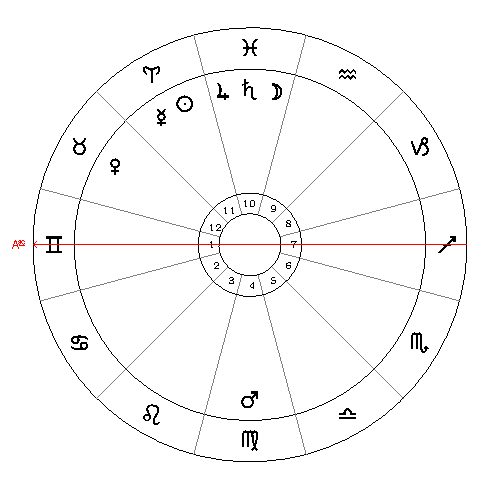
\includegraphics[width=0.7\textwidth]{charts/1_24_06}
\vspace{-1em}
\caption{Chart 06: Wealthy, an evil end}
\end{figure}

The nativity is diurnal and the triplicity rulers of the \Sun\, in \Aries\, are, first, the \Sun, second, \Jupiter, and third, \Saturn. As all three are in good places ``this man will abound in gold and silver'' but he will have an ``evil end'' because \Venus\, is the first triplicity ruler of the 4th ``from which the matter of the end and the situation of death are known'' and \Venus\,''is cadent in the sign of calamity\footnote{The 12th place.}.''

\newpage
\begin{figure}[H]
\centering
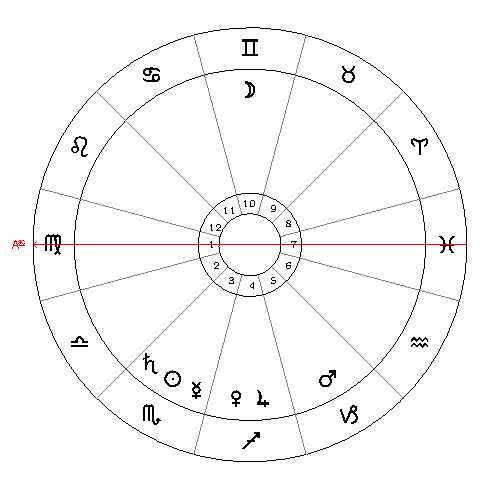
\includegraphics[width=0.7\textwidth]{charts/1_24_07}
\vspace{-1em}
\caption{Chart 07: Noble family but raised in poverty}
\end{figure}

The nativity is nocturnal and the triplicity rulers of the \Moon\, in \Gemini\, are, first, \Mercury, second, \Saturn, third, \Jupiter. The first and second are cadent, indicating ``poverty and indigence, and he will be beseeching all his days, but he will eat in misery...but since \Jupiter\, and \Venus\, are in cardines they indicate that he will be of noble lineage, but that he will be brought up and will grow up in houses of slavery, and he will curry favor with [his] brothers and nobles and will become acquainted [with them], but he will fail because of the evil effect of the lords of the \Moon's triplicity.''

\Mars\, ``indicates the loss of the property of his father and its dispersal in [all] directions''\footnote{Dykes, based on Pingree's timing for the chart, puts \Mars\, in the 2nd ``harming the native's assets'' but I believe the original also shows harm as \Mars, ruler of the 8th of inheritance in the 5th (risks) could indicate a sudden (\Mars\, exalted) loss (\Mars) of the father's assets (\Mars\, sextile \Saturn, \Sun) possibly due to his brothers (3rd) stealing them.}					% example charts
\section{Excellence of Fortune}
Indications of an increased fortune:
\begin{itemize}[topsep=0em,itemsep=0em]
\item triplicity ruler of the sect light in a good place in \Conjunction, \Opposition, \Trine, or \Square\, the \Moon

\item Asc, MC, and 2nd place rulers not malefic, angular or succedent, ``in their places with benefics'' then the person ``will possess fortune, eminence, commendation, praise, and a good livelihood
\end{itemize}

Indications of a middling fortune:
\begin{itemize}[topsep=0em,itemsep=0em]
\item a benefic in its domicile, exaltation, or triplicity, not USB or retrograde, with its triplicity ruler aspecting the ascendent but not the \Moon

\item rulers of the Asc, MC, and 2nd neither all in good or bad places
\end{itemize}

Indications of a bad fortune:
\begin{itemize}[topsep=0em,itemsep=0em]
\item the triplicity ruler of the sect averse to the ascendent, \Moon, the sect light and its dispositor, especially if \Jupiter, \Venus, and \Mercury\, are not in these places\footnote{Ascendant, place of \Moon, or sect light?} as it ``is more harmful and worse'' and indicates the person will not survive especially if \Saturn\, or \Mars\, are found there

\item rulers of the Asc, MC, and 2nd all cadent

\item rulers of all four angles (Asc, MC, 7th, 4th) and all four succedent (2nd, 8th, 11th, 5th) houses cadent with no aspect to the \Moon\, by night or \Sun\, by day, the person ``will be needing nourishment for his belly, and it will be worse for him if a malefic is in one of the cardines''
\end{itemize}
